\subsection{Secondo sprint}

\begin{minipage}{\textwidth}
Di seguito è riportata la distribuzione delle ore per ciascun membro del team, accumulate in totali per persona e per ruolo:
\begin{table}[H]
  \begin{tabularx}{\textwidth}{|c|*{6}{>{\centering}X|}c|}
    \hline
    \multicolumn{8}{|c|}{\textbf{Consuntivo orario}} \\
    \hline
    \textbf{Membro del team} & \textbf{Re} & \textbf{Am} & \textbf{An} & \textbf{Pt} & \textbf{Pr} & \textbf{Ve} & \textbf{Totale per persona} \\
    \hline
    Cavalli Riccardo & 1 & 6 & 0 & 0 & 0 & 0 & 7 \\
    \hline
    Pianon Raul & 7 & 0 & 0 & 0 & 0 & 0 & 7 \\
    \hline
    Dall'Amico Martina & 0 & 0 & 0 & 0 & 0 & 5 & 5 \\
    \hline
    Cristo Marco & 0 & 0 & 0 & 3 & 5 & 0 & 8 \\
    \hline
    Lewental Sebastiano & 0 & 0 & 0 & 6 & 0 & 0 & 6 \\
    \hline
    Zecchinato Mattia & 0 & 0 & 0 & 0 & 0 & 6 & 6 \\
    \hline
    Stocco Tommaso & 0 & 0 & 6 & 0 & 0 & 0 & 6 \\
    \hline
    \textbf{Totale per ruolo} & 8 & 6 & 6 & 9 & 5 & 11 & \textbf{45} \\
    \hline
  \end{tabularx}
  \caption{Sprint 2 - Consuntivo orario}
\end{table}
\end{minipage}

\begin{figure}[H]
  \centering
  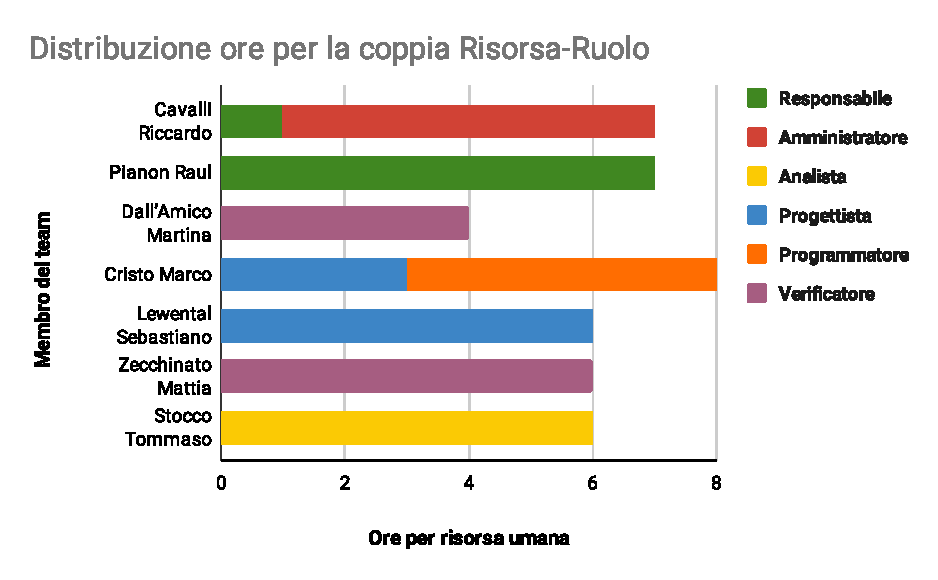
\includegraphics[width=0.90\textwidth]{assets/Consuntivo/Sprint-2/distribuzione_ore_risorsa_ruolo.pdf}
  \caption{Sprint 2 - Istogramma della distribuzione oraria per la coppia risorsa-ruolo}
\end{figure}

\begin{figure}[H]
  \centering
  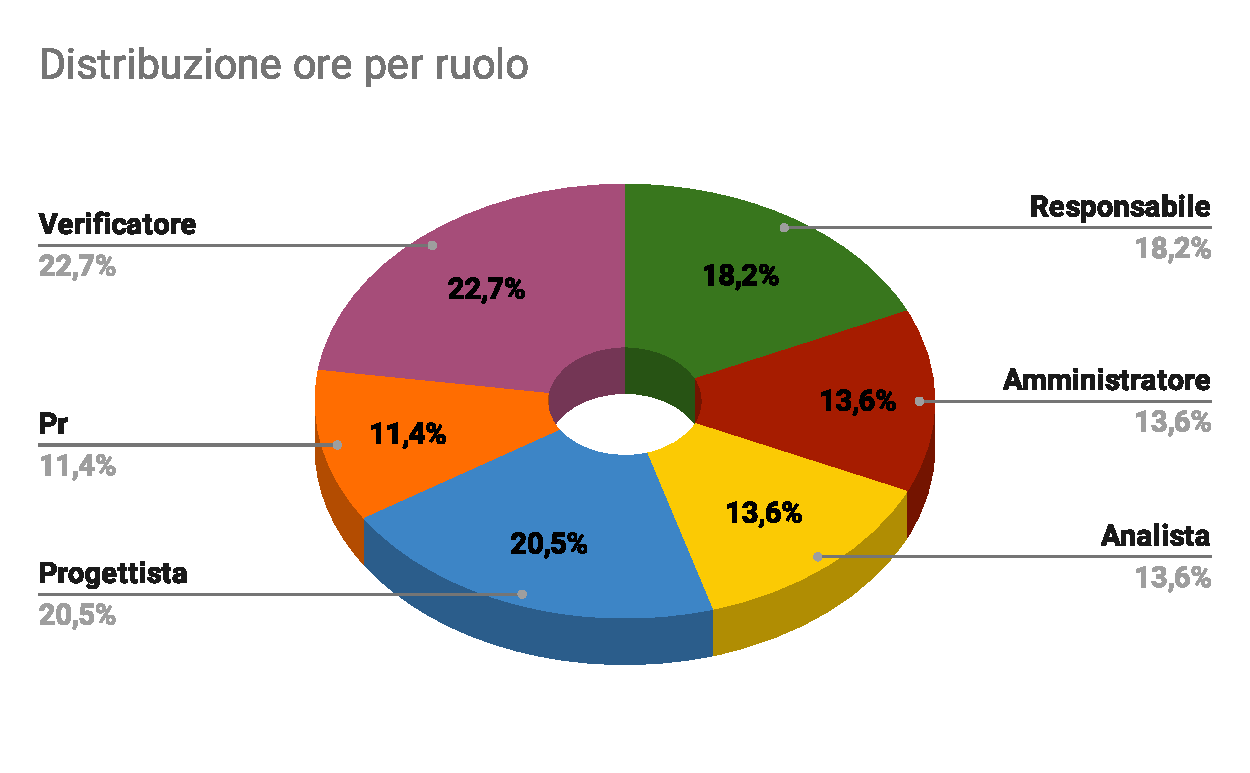
\includegraphics[width=0.90\textwidth]{assets/Consuntivo/Sprint-2/distribuzione_ore_ruolo.pdf}
  \caption{Sprint 2 - Areogramma della distribuzione oraria per ruolo}
\end{figure}

\begin{minipage}{\textwidth}
Di seguito è riportato il consuntivo economico del secondo \glossario{sprint}:
\begin{table}[H]
\begin{adjustwidth}{-0.5cm}{-0.5cm}
  \centering
  \begin{tabular}{|P{2.9cm}|P{2.3cm}|P{2.5cm}|P{2.3cm}|>{\arraybackslash}P{2.5cm}|}
    \hline
    \multicolumn{5}{|c|}{\textbf{Consuntivo economico}} \\
    \hline
    \textbf{Ruolo} & \textbf{Ore per ruolo} & \textbf{Delta ore preventivo - consuntivo} & \textbf{Costo (in \texteuro)} & \textbf{Delta costo preventivo - consuntivo (in \texteuro)} \\
    \hline
    Responsabile & 8 & +1 & 240,00 & +30,00 \\
    \hline
    Amministratore & 6 & -1 & 120,00 & -20,00 \\
    \hline
    Analista & 6 & -1 & 150,00 & -25,00 \\
    \hline
    Progettista & 9 & +2 & 225,00 & +50,00 \\
    \hline
    Programmatore & 5 & -3 & 75,00 & -45,00 \\
    \hline
    Verificatore & 11 & -1 & 160,00 & -15,00 \\
    \hline
    \textbf{Totale} & \textbf{45} & -3 & \textbf{975,00} & -25,00 \\
    \hline
    \textbf{Restante} & 542 & / & 10.870,00 & / \\
    \hline
    \textbf{Sprint pregressi} & 587 & / & 11.845,00 & / \\
    \hline
  \end{tabular}
  \caption{Sprint 2 - Consuntivo economico}
\end{adjustwidth}
\end{table}
\end{minipage}

\begin{figure}[H]
  \centering
  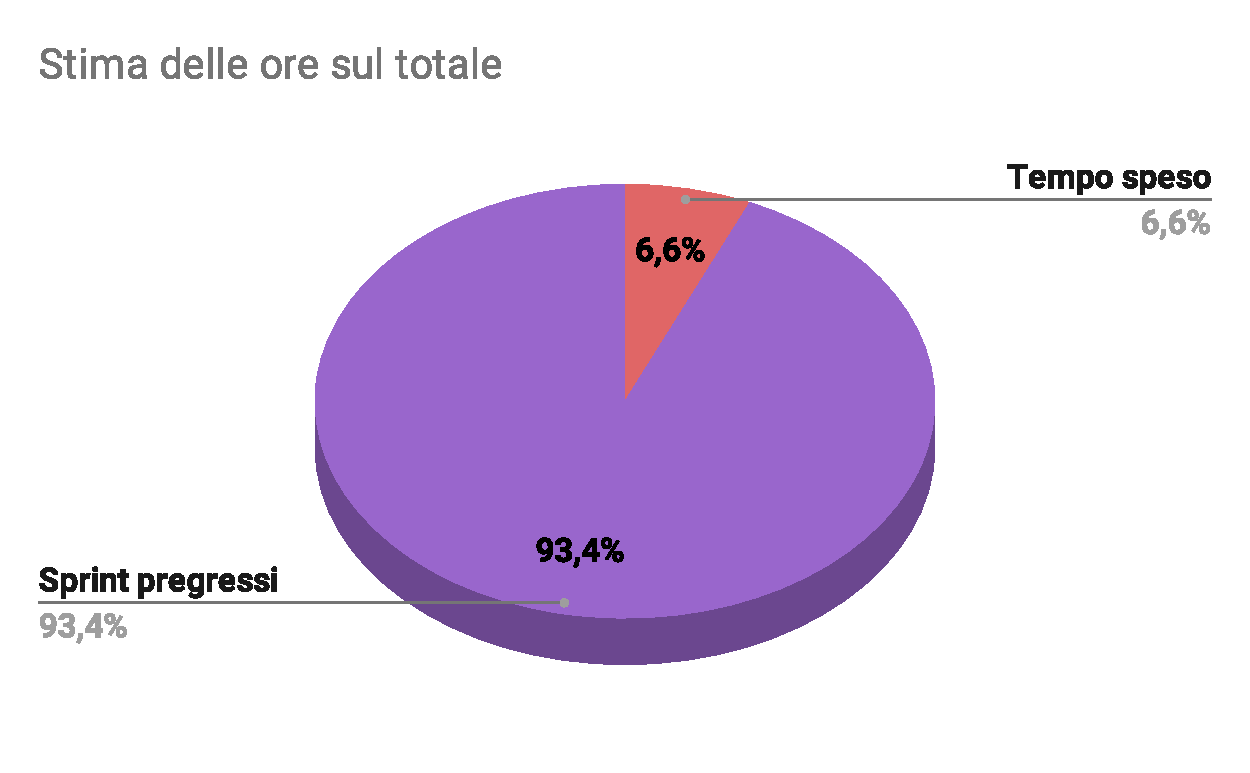
\includegraphics[width=0.90\textwidth]{assets/Consuntivo/Sprint-2/copertura_oraria.pdf}
  \caption{Sprint 2 - Areogramma del tempo speso (in ore) rispetto al totale}
\end{figure}

\begin{figure}[H]
  \centering
  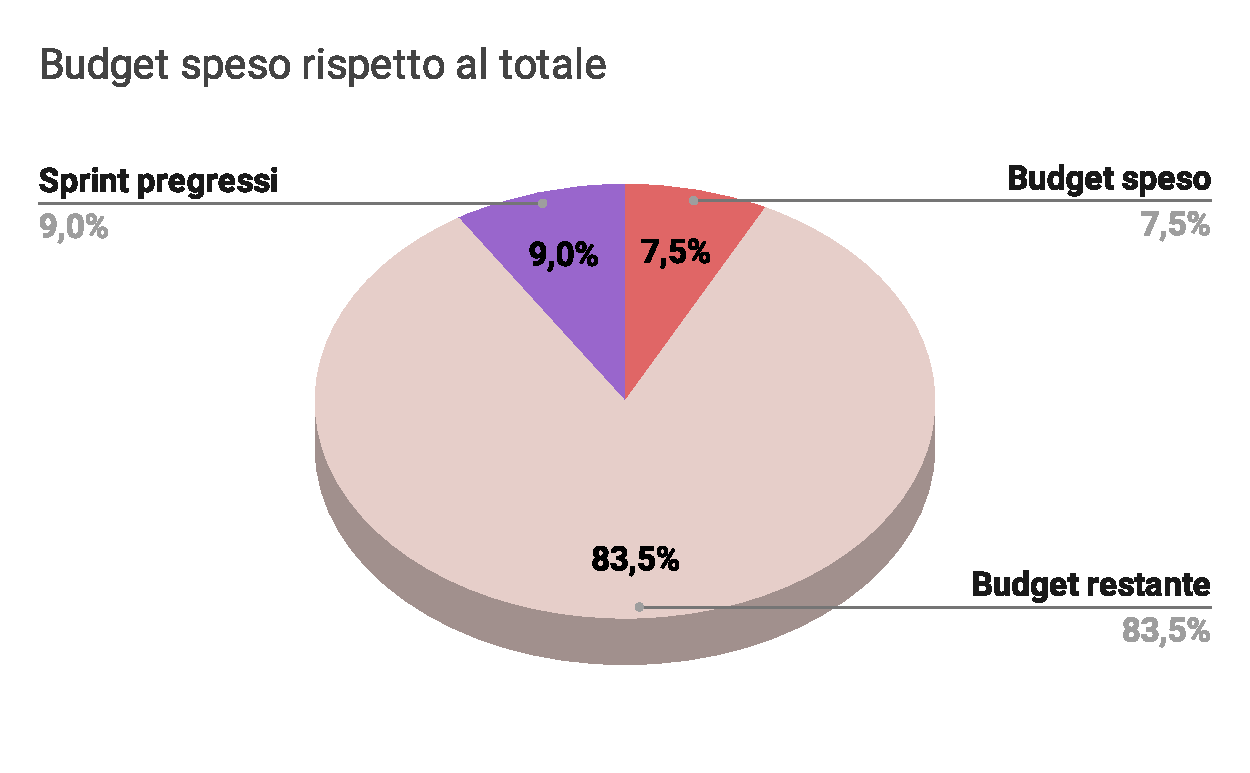
\includegraphics[width=0.90\textwidth]{assets/Consuntivo/Sprint-2/budget_speso.pdf}
  \caption{Sprint 2 - Areogramma del budget speso rispetto al totale}
\end{figure}

\begin{minipage}{\textwidth}
  Di seguito sono riportate le ore rimanenti per la coppia risorsa-ruolo:
  \begin{table}[H]
    \begin{tabularx}{\textwidth}{|c|*{6}{>{\centering}X|}c|}
      \hline
      \multicolumn{8}{|c|}{\textbf{Ore rimanenti per la coppia risorsa-ruolo}} \\
      \hline
      \textbf{Membro del team} & \textbf{Re} & \textbf{Am} & \textbf{An} & \textbf{Pt} & \textbf{Pr} & \textbf{Ve} & \textbf{Totale per persona} \\
      \hline
      Cavalli Riccardo & 1 & 2 & 9 & 23 & 22 & 20 & 77 \\
      \hline
      Pianon Raul & 2 & 8 & 9 & 23 & 22 & 12 & 76 \\
      \hline
      Dall'Amico Martina & 9 & 8 & 1 & 23 & 22 & 15 & 78 \\
      \hline
      Cristo Marco & 9 & 8 & 2 & 20 & 17 & 20 & 76 \\
      \hline
      Lewental Sebastiano & 9 & 8 & 2 & 17 & 22 & 20 & 78 \\
      \hline
      Zecchinato Mattia & 9 & 8 & 8 & 17 & 22 & 20 & 79 \\
      \hline
      Stocco Tommaso & 9 & 2 & 3 & 23 & 22 & 20 & 79 \\
      \hline
      \textbf{Totale per ruolo} & 48 & 44 & 34 & 146 & 149 & 121 & \textbf{542} \\
      \hline
    \end{tabularx}
    \caption{Sprint 2 - Ore rimanenti per la coppia risorsa-ruolo}
  \end{table}
\end{minipage}

\subsubsection{Revisione delle attività}

Nel corso del secondo \glossario{sprint}, il team ha svolto le seguenti attività:
\begin{itemize}
    \item Stesura Verbali Interni;
    \item Stesura Verbali Esterni;
    \item Stesura iniziale del \PdQ;
    \item Aggiornamento \PdP\ con l'aggiunta della sezione riguardante l'\ARischi, preventivi e consuntivi dei primi due \glossario{sprint};
    \item Aggiornamento del documento di \NdP\ con l'inserimento di una sezione riguardante \glossario{Jira Software}, l'integrazione con \glossario{GitHub}\ e la tabella dei ToDo;
    \item Popolamento del \Gls;
    \item Conversione del documento di \AdR\ in \glossario{LateX};
    \item Sistemazione dei Verbali Interni;
    \item Creazione di un template per la stesura degli appunti per i Verbali in GoogleDocs;
    \item Aggiornamento del documento di \AdR\ con l'espansione dei casi d'uso;
    \item Caricamento di file di configurazione per l'automatizzazione del caricamento dei pdf;
    \item Studio delle tecnologie;
    \item Ultimazione della stesura del \glossario{prompt};
    \item Studio delle tecnologie per lo sviluppo della \glossario{web app};
    \item Sviluppo di un prototipo per la parte funzionale del prodotto.
\end{itemize}

\subsubsection{Retrospettiva}

\par Di seguito sono riportati i risultati del questionario di valutazione dello \glossario{sprint}, realizzato dal Responsabile in carica per ottimizzare la fase di \glossario{retrospettiva}:
\begin{itemize}
  \item Organizzazione dello \glossario{sprint}\ - Valutazione: 8,5;
  \item Conduzione dei meeting interni - Valutazione: 8,5;
  \item Conduzione dei meeting esterni - Valutazione: 8,5;
  \item Impegno e partecipazione dei singoli membri - Valutazione: 7,5;
  \item Non tutti i membri del team erano a conoscenza delle proprie mansioni;
  \item La numerosità delle riunioni è adeguata;
  \item Le riunioni sono state organizzate quasi sempre con il giusto preavviso;
  \item Da migliorare significativamente il rapporto ore spese/ore produttive.
  \item Da migliorare la definizione del lavoro di Progettista e Programmatore
  \item Da migliorare la distribuzione delle risorse al ruolo di Amministratore
  \item Da definire meglio il ruolo del progettista 
  \item Proposta di divisione della stesura del \PdQ\ in sotto-task
\end{itemize}

\subsubsection{Aggiornamento pianificazione e preventivo}

\paragraph*{Pianificazione futura:}

\paragraph*{Preventivo "a finire" (\sezione{sec:stima_temporale}):}

\paragraph*{Gestione dei rischi (\sezione{sec:analisi_rischi}):}

